
\documentclass{article}
\usepackage{graphicx} % Required for inserting images
\usepackage{fancyhdr} % Required for header and footer configuration
\usepackage[a4paper, margin=2.5cm, left=1.5cm, right=1.5cm, bottom=4cm]{geometry} % Required for setting page margins
\usepackage[T1]{fontenc}
\usepackage[default,oldstyle,scale=1]{opensans} % Utilizzo del font Open Sans
\usepackage{lipsum}
\usepackage{makeidx}
\usepackage{booktabs}
\usepackage{tabularray}
\usepackage[colorlinks=true, linkcolor=black, urlcolor=blue, citecolor=blue]{hyperref}
\usepackage{tabularx}
\usepackage{makecell}
\usepackage{enumitem} % Pacchetto per la personalizzazione degli elenchi
\usepackage{booktabs}
\usepackage{subcaption}

% Configure header and footer for the first page
\fancypagestyle{firstpage}{
    \fancyhf{} % Clear header and footer
    \renewcommand{\headrulewidth}{0pt} % Remove header rule line
    \lhead{} % Header on the left
    \chead{} % Header in the center
    \rhead{} % Header on the right
    \lfoot{} % Footer on the left
    \cfoot{\vspace{5pt}\\\hrulefill\\\vspace{10pt}\textbf{BeeLive}\\Gruppo 21} % Footer in the center
    \rfoot{\vspace{32.5pt}\\\thepage} % Footer on the right
}

% Configure header and footer for non-plain pages (second page onwards)
\fancypagestyle{nonplain}{
    \fancyhf{} % Clear header and footer
    \lhead{} % Header on the left
    \chead{} % Header in the center
    \rhead{
\includegraphics[width=2cm]{Images/BeeLive-Logo.png}\\\vspace{2pt}} % Header on the right
    \lfoot{} % Footer on the left
    \cfoot{\vspace{5pt}\\\hrulefill\\\vspace{10pt}\textbf{BeeLive}\\Gruppo 21} % Footer in the center
    \rfoot{\vspace{32.5pt}\\\thepage} % Footer on the right
}

% Adjust vertical space between header and text                                    
\setlength{\headsep}{65pt} 
% Adjust vertical space between text and footer
\setlength{\footskip}{0pt} 

\title{
\includegraphics[width=0.75\textwidth]{Images/BeeLive-Logo.png}\\\vspace{100pt}
\LARGE{\textbf{BeeLive\\Deliverable 2}}}
\author{Gruppo 21:\\
Cipriani Pietro, 226959\\
Orlando Dennis, 227688\\
Ziviani Elia, 228172}
\date{22 Aprile 2024}

\makeindex % Indica che vogliamo creare un indice

\begin{document}

\maketitle
\thispagestyle{firstpage} % Apply firstpage style to the first page
\clearpage

\pagestyle{nonplain} % Apply non-plain style to subsequent pages

\renewcommand{\contentsname}{Indice}
\tableofcontents

\clearpage

\section{Component Diagram}
\index{Component Diagram}

Questo capitolo è incentrato sull'analisi dei componenti del sistema che saranno realizzati.\\
Lo scopo è quello di descrivere ogni singolo componente in termini di funzionalità e interfacce.\\

I componenti sono individuati seguendo quando espresso nel documento Deliverable 1 per quanto riguarda i casi d'uso e sono definiti come entità autonome nel sistema.\\
Questi componenti sono provvisti di interfacce che permettono la comunicazione tra di essi.\\
Le interfacce sono definite come:
\begin{itemize}
    \item \textbf{Interfacce di OUTPUT}: Tutte quelle interfacce che offrono servizi al sistema.
    \item \textbf{Interfacce di INPUT}: Tutte quelle interfacce che ricevono servizi dal sistema.
\end{itemize} 

\begin{figure}[htbp]
    \centering
    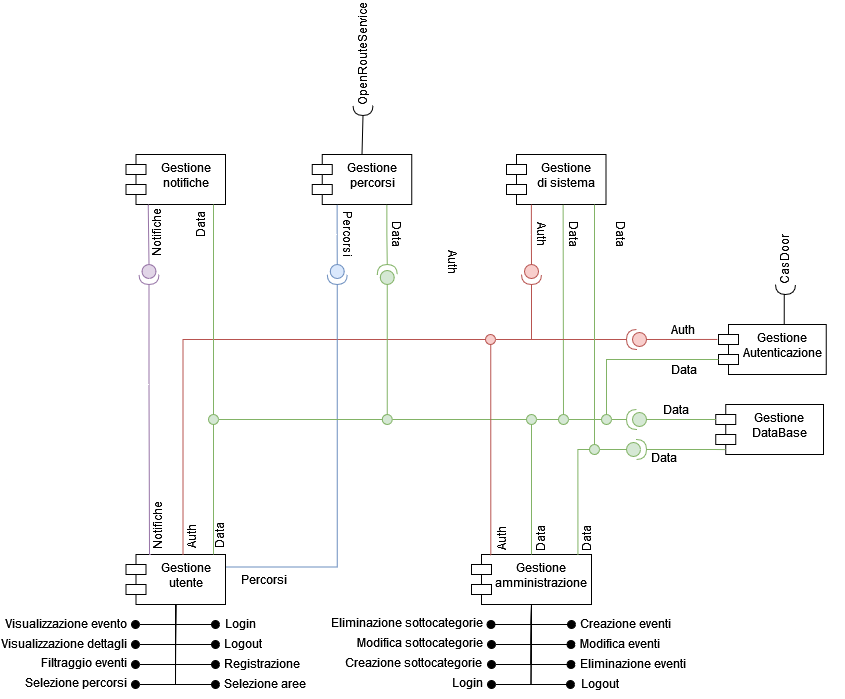
\includegraphics[width=1\textwidth]{Images/ComponentDiagram.png}
    \caption{Diagramma dei componenti}
    \label{fig:component-diagram}
\end{figure}

\clearpage

\subsection{Gestione utente}
\index{Gestione utente}

\begin{table}[htbp]
    \centering
    \renewcommand{\arraystretch}{1.3} % Imposta lo spazio verticale delle righe
    \begin{tabularx}{\textwidth}{| l | l | X |}
        \Xhline{2pt}
        \textbf{INPUT} & \textbf{Nome} & \textbf{Descrizione} \\
        \Xhline{2pt}
         & Notifiche & Il componente utilizza l'interfaccia fornita dal componente "Gestione Notifiche" per ricevere notifiche relative alle criticita' \\
        \hline
         & Auth & Il componente utilizza l'interfaccia fornita dal componente "Gestione Autenticazione" per richiedere il token necessario per effettuare il login \\
        \hline
         & Data & Il componente utilizza l'interfaccia fornita dal componente di gestione del database per scambiare tutti i dati necessari a garantire un corretto funzionamento dell'applicativo per gli utenti \\
        \hline
         & Percorsi & Il componente utilizza l'interfaccia fornita dal componente gestione percorsi per ottenere i percorsi calcolati evitando le criticità presenti in mappa \\
        \Xhline{2pt}
        \textbf{OUTPUT} & \textbf{Nome} & \textbf{Descrizione} \\
        \Xhline{2pt}
         & Login & Il componente fornisce un'interfaccia per effettuare il login attraverso i servizi del componente esterno CasDoor, che prevede l'inserimento delle specifiche credenziali per generare un token di accesso \\
        \hline
         & Logout & Il componente fornisce all'utente un'interfaccia per effettuare il logout \\
        \hline
         & Registrazione & Il componente fornisce all'utente un'interfaccia per registrarsi attraverso il servizio CasDoor \\
        \hline
         & Selezione aree & Il componente fornisce un'interfaccia che permette all'utente di specificare sulla mappa della citta' di Trento la sua zona di maggior interesse per poi considerare quella zona come utile per la visualizzazione dei dati \\
        \hline
         & Visualizzazione evento & Il componente fornisce un'interfaccia che permette la visualizzazione di tutti gli eventi presenti sul database riguardanti la citta' di Trento o la zona/il percorso d'interesse se specificati \\
        \hline
         & Visualizzazione dettagli & Il componente offre un'interfaccia per la visualizzazione di tutti i dettagli che caratterizzano il singolo evento selezionato \\
        \hline
         & Filtraggio eventi & E' offerta dal componente l'interfaccia che permette il filtraggio degli eventi tramite specificita' espresse dall'utilizzatore \\
        \hline
         & Selezione aree & Il componente offre l'interfaccia per la specifica delle aree di maggiore interesse secondo l'utente. Questa specifica e' utile per la visualizzazione delle sole criticita' contenute in essa \\
        \hline
         & Selezione percorsi & Il componente offre l'interfaccia per la specifica dei percorsi piu' significativi per l'utente permettendogli di essere notificato nel caso in cui nel percorso si verifichi una criticita' \\
        \hline
    \end{tabularx}
    \caption{Tabella gestione utente}
\end{table}

\clearpage

\subsection{Gestione amministrazione}
\index{Gestione amministrazione}

\begin{table}[htbp]
    \centering
    \renewcommand{\arraystretch}{1.3} % Imposta lo spazio verticale delle righe
    \begin{tabularx}{\textwidth}{| l | l | X |}
        \Xhline{2pt}
        \textbf{INPUT} & \textbf{Nome} & \textbf{Descrizione} \\
        \Xhline{2pt}
         & Auth & Il componente utilizza l'interfaccia fornita dal componente "Gestione Autenticazione" per richiedere il token necessario per effettuare il login \\
        \hline
         & Data & Il componente utilizza l'interfaccia fornita dal componente di gestione del database per scambiare tutti i dati necessari a garantire un corretto funzionamento dell'applicativo per l'amministrazione, come il salvataggio delle operazioni eseguite sugli eventi \\
        \Xhline{2pt}
        \textbf{OUTPUT} & \textbf{Nome} & \textbf{Descrizione} \\
        \Xhline{2pt}
         & Creazione eventi & Il componente offre internamente l'interfaccia per la creazione di un nuovo evento, seguendo e verificando che le informazioni utilizzate siano corrette \\
        \hline
         & Modifica eventi & Il componente offre internamente l'interfaccia utile alla modifica degli eventi gia' pubblicati e salvati in precedenza su database \\
        \hline
         & Eliminazione eventi & Il componente prevede internamente l'interfaccia che si occupa di eseguire le operazioni di eliminazione degli eventi pubblicati e salvati su database \\
        \hline
         & Creazione sottocategorie & Il componente offre internamente l'interfaccia che permette all'amministrazione di creare nuove sottocategorie degli eventi, fornendo una migliore organizzazione degli stessi \\
        \hline
         & Modifica sottocategorie & Il componente offre internamente l'interfaccia per eseguire modifiche sulle sottocategorie create e salvate su database \\
        \hline
         & Eliminazione sottocategorie & Il componente offre internamente l'interfaccia per permettere la cancellazione delle sottocategorie create e salvate su database in precedenza \\
        \hline
         & Data & Il componente utilizza questa interfaccia per eseguire il caricamento e il salvataggio dei nuovi dati di eventi e categorie su database \\
        \hline
    \end{tabularx}
    \caption{Tabella gestione amministrazione}
\end{table}

\clearpage

\subsection{Gestione di sistema}
\index{Gestione di sistema}

\begin{table}[htbp]
    \centering
    \renewcommand{\arraystretch}{1.3} % Imposta lo spazio verticale delle righe
    \begin{tabularx}{\textwidth}{| l | l | X |}
        \Xhline{2pt}
        \textbf{INPUT} & \textbf{Nome} & \textbf{Descrizione} \\
        \Xhline{2pt}
         & Data & Il componente utilizza un’interfaccia fornita dal datalayer per accedere ai dati sul database \\
        \hline
         & Auth & Il componente utilizza l'interfaccia fornita dal componente "Gestione Autenticazione" per richiedere il token necessario per effettuare il login \\
         \Xhline{2pt}
        \textbf{OUTPUT} & \textbf{Nome} & \textbf{Descrizione} \\
        \Xhline{2pt}
         & Data & Il componente fornisce internamente un’interfaccia per accedere al database \\
        \hline
         & Gestione competenze & Il componente fornisce internamente un'interfaccia per la gestione delle aree di competenza degli utenti \\
        \hline
         & Gestione access policies & Il componente fornisce internamente un'interfaccia utile alla gestione delle access policies degli utenti nel sistema \\
        \hline
        \end{tabularx}
    \caption{Tabella gestione di sistema}
\end{table}

\subsection{Gestione autenticazione}
\index{Gestione autenticazione}

\begin{table}[htbp]
    \centering
    \renewcommand{\arraystretch}{1.3} % Imposta lo spazio verticale delle righe
    \begin{tabularx}{\textwidth}{| l | l | X |}
        \Xhline{2pt}
        \textbf{INPUT} & \textbf{Nome} & \textbf{Descrizione} \\
        \Xhline{2pt}
         & CasDoor & Il componente utilizza l'interfaccia fornita da CasDoor per l'autenticazione degli utenti. CasDoor e' un servizio specifico negli accessi degli utenti \\
        \hline
         & Data & Il componente utilizza l’interfaccia del componente "Gestione database" per autenticare gli utenti registrati \\
        \Xhline{2pt}
        \textbf{OUTPUT} & \textbf{Nome} & \textbf{Descrizione} \\
        \Xhline{2pt}
         & Auth & Il componente fornisce un'interfaccia agli altri componenti per usufruire del token generato all'accesso nei servizi previsti, in risposta all’inserimento dei dati accesso e alla loro validazione \\
        \hline
    \end{tabularx}
    \caption{Tabella gestione autenticazione}
\end{table}

\clearpage

\subsection{Gestione notifiche}
\index{Gestione notifiche}

\begin{table}[htbp]
    \centering
    \renewcommand{\arraystretch}{1.3} % Imposta lo spazio verticale delle righe
    \begin{tabularx}{\textwidth}{| l | l | X |}
        \Xhline{2pt}
        \textbf{INPUT} & \textbf{Nome} & \textbf{Descrizione} \\
        \Xhline{2pt}
         & Data & Il componente utilizza un'interfaccia fornita dal datalayer per accedere ai dati sul database \\
        \Xhline{2pt}
        \textbf{OUTPUT} & \textbf{Nome} & \textbf{Descrizione} \\
        \Xhline{2pt}
         & Notifiche & Il componente fornisce internamente un'interfaccia per l'inoltro delle notifiche \\
        \hline
    \end{tabularx}
    \caption{Tablla gestione notifiche}
\end{table}

\subsection{Gestione percorsi}
\index{Gestione percorsi}

\begin{table}[htbp]
    \centering
    \renewcommand{\arraystretch}{1.3} % Imposta lo spazio verticale delle righe
    \begin{tabularx}{\textwidth}{| l | l | X |}
        \Xhline{2pt}
        \textbf{INPUT} & \textbf{Nome} & \textbf{Descrizione} \\
        \Xhline{2pt}
         & Data & Il componente utilizza un'interfaccia fornita dal datalayer per accedere ai dati sul database  \\
        \hline
         & OpenRouteService & Il componente utilizza un'interfaccia fornita dal servizio OpenRouteService per il calcolo dei percorsi \\
         \Xhline{2pt}
        \textbf{OUTPUT} & \textbf{Nome} & \textbf{Descrizione} \\
        \Xhline{2pt}
         & Percorsi & Il componente fornisce internamente un'interfaccia per la computazione dei percorsi che evitano le zone con criticita' di viabilita' \\
        \hline
    \end{tabularx}
    \caption{Tabella gestione percorsi}
\end{table}

\subsection{Gestione database}
\index{Gestione database}

\begin{table}[htbp]
    \centering
    \renewcommand{\arraystretch}{1.3} % Imposta lo spazio verticale delle righe
    \begin{tabularx}{\textwidth}{| l | l | X |}
        \Xhline{2pt}
        \textbf{INPUT} & \textbf{Nome} & \textbf{Descrizione} \\
        \Xhline{2pt}
         & Data & Il componente utilizza un’interfaccia fornita dal datalayer per accedere ai dati sul database \\
        \Xhline{2pt}
        \textbf{OUTPUT} & \textbf{Nome} & \textbf{Descrizione} \\
        \Xhline{2pt}
         & Data & Il componente fornisce internamente un’interfaccia per accedere al database \\
        \hline
    \end{tabularx}
    \caption{Tabella gestione database}
\end{table}

\clearpage

\section{Diagramma delle classi}
\index{Diagramma delle classi}

Nella sezione seguente verranno descritte nel dettaglio le classi che formeranno la struttura del sistema attraverso il diagramma delle classi.\\
Saranno quindi descritte, oltre alle classi, anche tutte le relazioni che intercorrono tra di esse e i ruoli dei gestori.\\

La descrizione sarà divisa, per motivi di chiarezza, in due sezioni. La prima tratterà le classi relative agli utenti, mentre la seconda tratterà le rimanenti.\\

\subsection{Utenti}
\index{Utenti}

\subsubsection{Utente}
\index{Utente}

\begin{figure}[htbp]
    \centering
    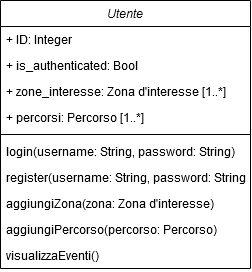
\includegraphics[width=0.25\textwidth]{Images/utente_class.png}
    \caption{Classe Utente}
    \label{fig:utente}
\end{figure}

Questa classe rappresenta la figura dell'utente che utilizza l'applciazione mobile senza seguire la procedura di autenticazione.\\
Come riportato nel primo documento "Deliverable 1" nella sezione relativa agli attori [Ref. 3.1.1, pag. 6], l'utente non autenticato ha accesso a tutte le funzionalità dell'applicazione salvando lo stato solamente sul dispositivo su cui è installata l'applicazione, quindi perdendo i dati una volta cambiato dispositivo.\\

\textbf{Attributi:}\\

Gli attributi che caratterizzano questa classe sono:
\begin{itemize}
    \item \textbf{ID}: Attributo che rappresenta univocamente l'utente non autenticato.
    \item \textbf{is\_authenticated}: Questo attributo definisce se l'utente è autenticato o meno. Per l'utente non autenticato il valore sarà "False".
    \item \textbf{zone\_interesse}: Attributo che rappresenta la zona di interesse impostate dall'utente.
    \item \textbf{percorsi}: Attributo che rappresenta i percorsi che per l'utente risultano di interesse.
\end{itemize}
 
\clearpage

\textbf{Metodi:}\\

I metodi a disposizione della classe sono:
\begin{itemize}
    \item \textbf{login(username, password)}: Metodo utilizzato per effettuare il login all'interno dell'applicazione. Utilizzando questo metodo l'utente diventa un "Utente autenticato".\\Sono utilizzati metodi del gestore "Gestione utente" e del gestore "Gestione autenticazione" per effettuare il login.
    \item \textbf{register(username, password)}: Metodo che permette all'utente di registrarsi per la prima volta all'interno dell'applicazione.\\Sono utilizzati metodi del gestore "Gestione utente" e del gestore "Gestione autenticazione" per effettuare la registrazione. Anche questo metodo fa diventare l'utente un "Utente autenticato".
    \item \textbf{aggiungiZona(zona)}: Metodo utilizzato dall'utente per selezionare la zona di interesse sulla mappa.\\
    \item \textbf{aggiungiPercorso(percorso):} Metodo che permette all'utente di selezionare il percorso di interesse sulla mappa.
    \item \textbf{visualizzaEventi()}: Metodo utilizzato per visualizzare gli eventi presenti sulla mappa o all'interno della zona d'interesse precedentemente specificata.
\end{itemize} 

\subsubsection{Utente autenticato}
\index{Utente autenticato}

\begin{figure}[htbp]
    \centering
    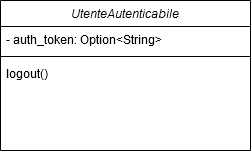
\includegraphics[width=0.25\textwidth]{Images/utenteAut_class.png}
    \caption{Classe Utente Autenticato}
    \label{fig:utente_autenticato}
\end{figure}

L'utente autenticato [Ref. 3.1.2, pag. 6] deriva le sue caratteristiche dall'utente non autenticato, ma ha la possibilità di salvare i dati sul server permettendo quindi di mantenere lo stato dell'applicazione anche cambiando dispositivo.\\

\textbf{Attributi:}\\
Sono gli stessi a disposizione dell'utente non autenticato, con l'aggiunta di:
\begin{itemize}
    \item \textbf{auth\_token}: Attributo che rappresenta il token di autenticazione dell'utente.
\end{itemize}

\textbf{Metodi:}\\
Anche i metodi sono gli stessi a disposizione dell'utente non autenticato, aggiungendo però il metodo:
\begin{itemize}
    \item \textbf{logout()}: Metodo utilizzato per effettuare il logout dall'applicazione.\\Sono utilizzati metodi del gestore "Gestione utente" e del gestore "Gestione autenticazione" per effettuare il logout.
\end{itemize}
Ed eliminando la possibilita' di richiamare i metodi "login" e "register", superflui in quanto l'utente è già autenticato.

\clearpage

\subsubsection{Utente amministratore}
\index{Utente amministratore}

\begin{figure}[htbp]
    \centering
    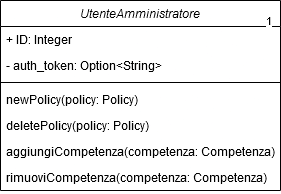
\includegraphics[width=0.3\textwidth]{Images/utenteAmministratore_class.png}
    \caption{Classe Utente Amministratore}
    \label{fig:utente_amministratore}
\end{figure}

L'utente amministratore [Ref. 3.1.4, pag. 6] è la classe che rappresenta l'utente che ha il controllo totale sul sistema, con la possibilita' di definire competenze e policy di accesso per gli utenti.

\textbf{Attributi:}\\
Gli attributi che caratterizzano questa classe sono:
\begin{itemize}
    \item \textbf{ID}: Attributo che identifica univocamente l'utente amministratore.
    \item \textbf{auth\_token}: Attributo che rappresenta il token di autenticazione dell'utente.
\end{itemize}

\textbf{Metodi:}\\
I metodi a disposizione della classe sono:

\begin{itemize}
    \item \textbf{login(username, password)}: Metodo utilizzato per effettuare il login all'interno dell'applicazione. Utilizzando questo metodo l'utente diventa un "Utente autenticato".\\Sono utilizzati metodi del gestore "Gestione utente" e del gestore "Gestione autenticazione" per effettuare il login.
    \item \textbf{logout(username, password)}: Metodo utilizzato per effettuare il logout dall'applicazione, cosi' da disconnettere l'utente dal servizio
    \item \textbf{aggiungiPolicy(policy)}: Metodo che permette all'utente amministratore di definire le policy di accesso per gli utenti.
    \item \textbf{rimuoviPolicy(policy)}: Metodo che permette all'utente amministratore di rimuovere le policy di accesso per gli utenti.
    \item \textbf{aggiungiCompetenza(competenza)}: Metodo che permette all'utente amministratore di definire le competenze degli utenti.
    \item \textbf{rimuoviCompetenza(competenza)}: Metodo che permette all'utente amministratore di rimuovere le competenze degli utenti.
\end{itemize}

\clearpage

\subsubsection{Utente autorizzato}
\index{Utente autorizzato}

\begin{figure}[htbp]
    \centering
    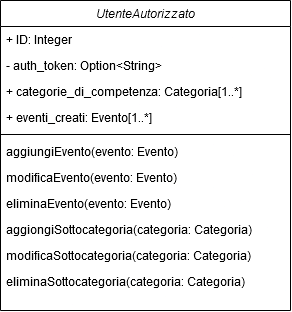
\includegraphics[width=0.275\textwidth]{Images/utenteAutorizzato_class.png}
    \caption{Classe Utente Autorizzato}
    \label{fig:utente_autorizzato}
\end{figure}

L'utente autorizzato [Ref. 3.1.3, pag. 6] è la classe che rappresenta tutte le entita' comunali che hanno i permessi di inserire gli eventi a sistema.\\
Questi utenti accedono al sistema attraverso l'applicativo desktop, sviluppato apposta per la gestione degli eventi.\\

\textbf{Attributi:}\\
Gli attributi che definiscono questa classe sono:
\begin{itemize}
    \item \textbf{ID}: Caratteristica che identifica univocamente l'utente autorizzato nel sistema.
    \item \textbf{auth\_token}: Attributo che rappresenta il token di autenticazione dell'utente.
    \item \textbf{categorie\_di\_competenza}: Riporta le categorie su cui l'utente ha competenza.
    \item \textbf{eventi\_creati}: Tutti gli eventi che l'utente ha creato e salvato sul database.
\end{itemize}

\textbf{Metodi:}\\
I metodi a disposizione della classe sono:
\begin{itemize}
    \item \textbf{login(username, password)}: Metodo utilizzato per effettuare il login all'interno dell'applicazione. Utilizzando questo metodo l'utente diventa un "Utente autenticato".\\Sono utilizzati metodi del gestore "Gestione utente" e del gestore "Gestione autenticazione" per effettuare il login.
    \item \textbf{logout(username, password)}: Metodo utilizzato per effettuare il logout dall'applicazione, cosi' da disconnettere l'utente dal servizio
    \item \textbf{aggiungiEvento(evento)}: Metodo che permette all'utente autorizzato di creare ed aggiungere un evento al sistema.
    \item \textbf{modificaEvento(evento)}: Metodo che permette all'utente autorizzato di modificare ed aggiornare un evento precedentemente creato.
    \item \textbf{eliminaEvento(evento)}: Metodo che permette all'utente autorizzato di eliminare dal sistema un evento precedentemente creato.
    \item \textbf{aggiongiSottocategoria(categoria)}: Metodo che permette all'utente autorizzato di creare ed aggiungere una sottocategoria di eventi al sistema.
    \item \textbf{modificaSottocategoria(categoria)}: Metodo che permette all'utente autorizzato di modificare ed aggiornare una sottocategoria di eventi precedentemente creata.
    \item \textbf{eliminaSottocategoria(categoria)}: Metodo che permette all'utente autorizzato di eliminare dal sistema una sottocategoria di eventi precedentemente creata.
\end{itemize}

\clearpage

\subsection{Altre classi}
\index{Altre classi}

\subsubsection{Evento}
\index{Evento}

\begin{figure}[htbp]
    \centering
    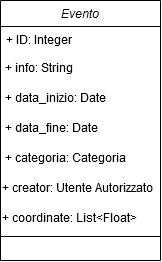
\includegraphics[width=0.15\textwidth]{Images/evento_class.png}
    \caption{Classe Evento}
    \label{fig:evento}
\end{figure}

La classe "Evento" rappresenta un evento o criticita' che l'utente amministratore pubblica sul sistema e che e' possibile visualizzare da applicativo mobile.

\textbf{Attributi:}\\
\begin{itemize}
    \item \textbf{ID}: Attributo che identifica univocamente l'evento pubblicato sul sistema.
    \item \textbf{titolo}: Attributo che rappresenta il titolo dell'evento.
    \item \textbf{descrizione}: Attributo che rappresenta la descrizione dell'evento.
    \item \textbf{data\_inizio}: Attributo che riporta la data d'inizio dell'evento.
    \item \textbf{data\_inizio}: Attributo che riporta la data di fine dell'evento.
    \item \textbf{categoria}: Attributo che rappresenta la categoria a cui l'evento appartiene.
    \item \textbf{creator}: Attributo che rappresenta l'utente autorizzato che ha creato l'evento.
    \item \textbf{coordinate}: Attributo che rappresenta il luogo in cui l'evento si svolgera'.\\
\end{itemize}
Per la classe in questione non sono previsti metodi.

\clearpage 

\subsubsection{Percorso}
\index{Percorso}

\begin{figure}[htbp]
    \centering
    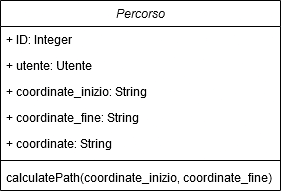
\includegraphics[width=0.25\textwidth]{Images/percorso_class.png}
    \caption{Classe Percorso}
    \label{fig:percorso}
\end{figure}

La classe "Percorso" rappresenta un percorso che l'utente richiede di calcolare da un punto d'inizio ad un punto di fine.\\
Il percorso che risulta rappresenta la via per raggiungere il punto di destinazione evitando tutte le criticita' presenti su mappa.\\

\textbf{Attributi:}\\
Gli attributi che caratterizzano questa classe sono:
\begin{itemize}
    \item \textbf{ID}: Attributo che identifica univocamente il percorso richiesto dall'utente.
    \item \textbf{utente}: Attributo che rappresenta univocamente l'utente che ha richiesto il percorso.
    \item \textbf{coordinate\_inizio}: Attributo che rappresenta le coordinate del punto di partenza del percorso.
    \item \textbf{coordinate\_fine}: Attributo che rappresenta le coordinate del punto di arrivo del percorso.
    \item \textbf{coordinate}: Attributo che rappresenta tutte le coordinate tra il punto di partenza e di arrivo del percorso, una volta che e' stato calcolato per evitare situazioni critiche su mappa.
\end{itemize}

\textbf{Metodi:}\\
Il metodo a disposizione della classe è:
\begin{itemize}
    \item \textbf{calcolaPercorso(coordinate\_inizio, coordinate\_fine)}: Metodo invocato per eseguire il calcolo del percorso dal punto di partenza al punto di arrivo evitando tutte le criticita' presenti su mappa.
\end{itemize}

\clearpage

\subsubsection{Zone di interesse}
\index{Zone di interesse}

\begin{figure}[htbp]
    \centering
    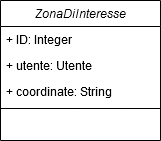
\includegraphics[width=0.175\textwidth]{Images/zona_class.png}
    \caption{Classe Zona di Interesse}
    \label{fig:zona}
\end{figure}

La classe "Zone di interesse" rappresenta le zone che l'utente ha selezionato come di interesse per la visualizzazione degli eventi e delle criticita' presenti su mappa.\\

\textbf{Attributi:}\\
Gli attributi che caratterizzano questa classe sono:
\begin{itemize}
    \item \textbf{ID}: Attributo che identifica univocamente la zona di interesse selezionata dall'utente.
    \item \textbf{utente}: Attributo che rappresenta univocamente l'utente che ha selezionato la zona di interesse.
    \item \textbf{coordinate}: Attributo che rappresenta le coordinate della zona di interesse selezionata dall'utente.\\
\end{itemize}
Per la classe in questione non sono previsti metodi.

\subsubsection{Categoria}
\index{Categoria}

\begin{figure}[htbp]
    \centering
    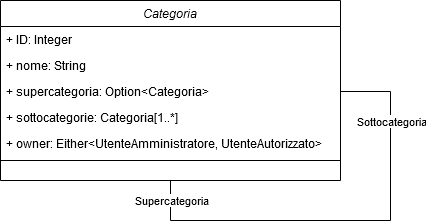
\includegraphics[width=0.45\textwidth]{Images/categoria_class.png}
    \caption{Classe Categoria}
    \label{fig:categoria}
\end{figure}

La classe "Categoria" rappresenta le categorie di eventi presenti sul sistema, definibili dagli utenti autorizzati dal comune di Trento.\\

\textbf{Attributi:}\\
Gli attributi che caratterizzano questa classe sono:
\begin{itemize}
    \item \textbf{ID}: Attributo che identifica univocamente la categoria di eventi.
    \item \textbf{nome}: Attributo che rappresenta il nome della categoria di eventi.
    \item \textbf{supercategoria}: Attributo che rappresenta la supercategoria a cui la categoria appartiene.
    \item \textbf{sottocategorie}: Attributo che rappresenta le sottocategorie di eventi presenti nella categoria.
    \item \textbf{owner}: Attributo che rappresenta l'utente autorizzato che ha creato la categoria.\\
\end{itemize}
Per la classe in questione non sono previsti metodi.

\subsubsection{Competenza}
\index{Competenza}

La classe "Competenza" rappresenta le competenze degli utenti autorizzati per la gestione degli eventi.\\

\textbf{Attributi:}\\
Gli attributi che caratterizzano questa classe sono:
\begin{itemize}
    \item \textbf{ID}: Attributo che identifica univocamente la competenza dell'utente.
    \item \textbf{id\_utente}: Attributo che rappresenta univocamente l'utente autorizzato che ha la competenza.
\end{itemize}

Da definire

\subsubsection{Policy}
\index{Policy}

La classe "Policy" rappresenta le policy di accesso degli utenti al sistema.\\

\textbf{Attributi:}\\
Gli attributi che caratterizzano questa classe sono:
\begin{itemize}
    \item \textbf{ID}: Attributo che identifica univocamente la policy di accesso.
    \item \textbf{nome}: Attributo che rappresenta il nome della policy di accesso.
    \item \textbf{utenti}: Attributo che rappresenta gli utenti autorizzati che seguono la policy.
\end{itemize}

\clearpage

\begin{figure}[htbp]
    \centering
    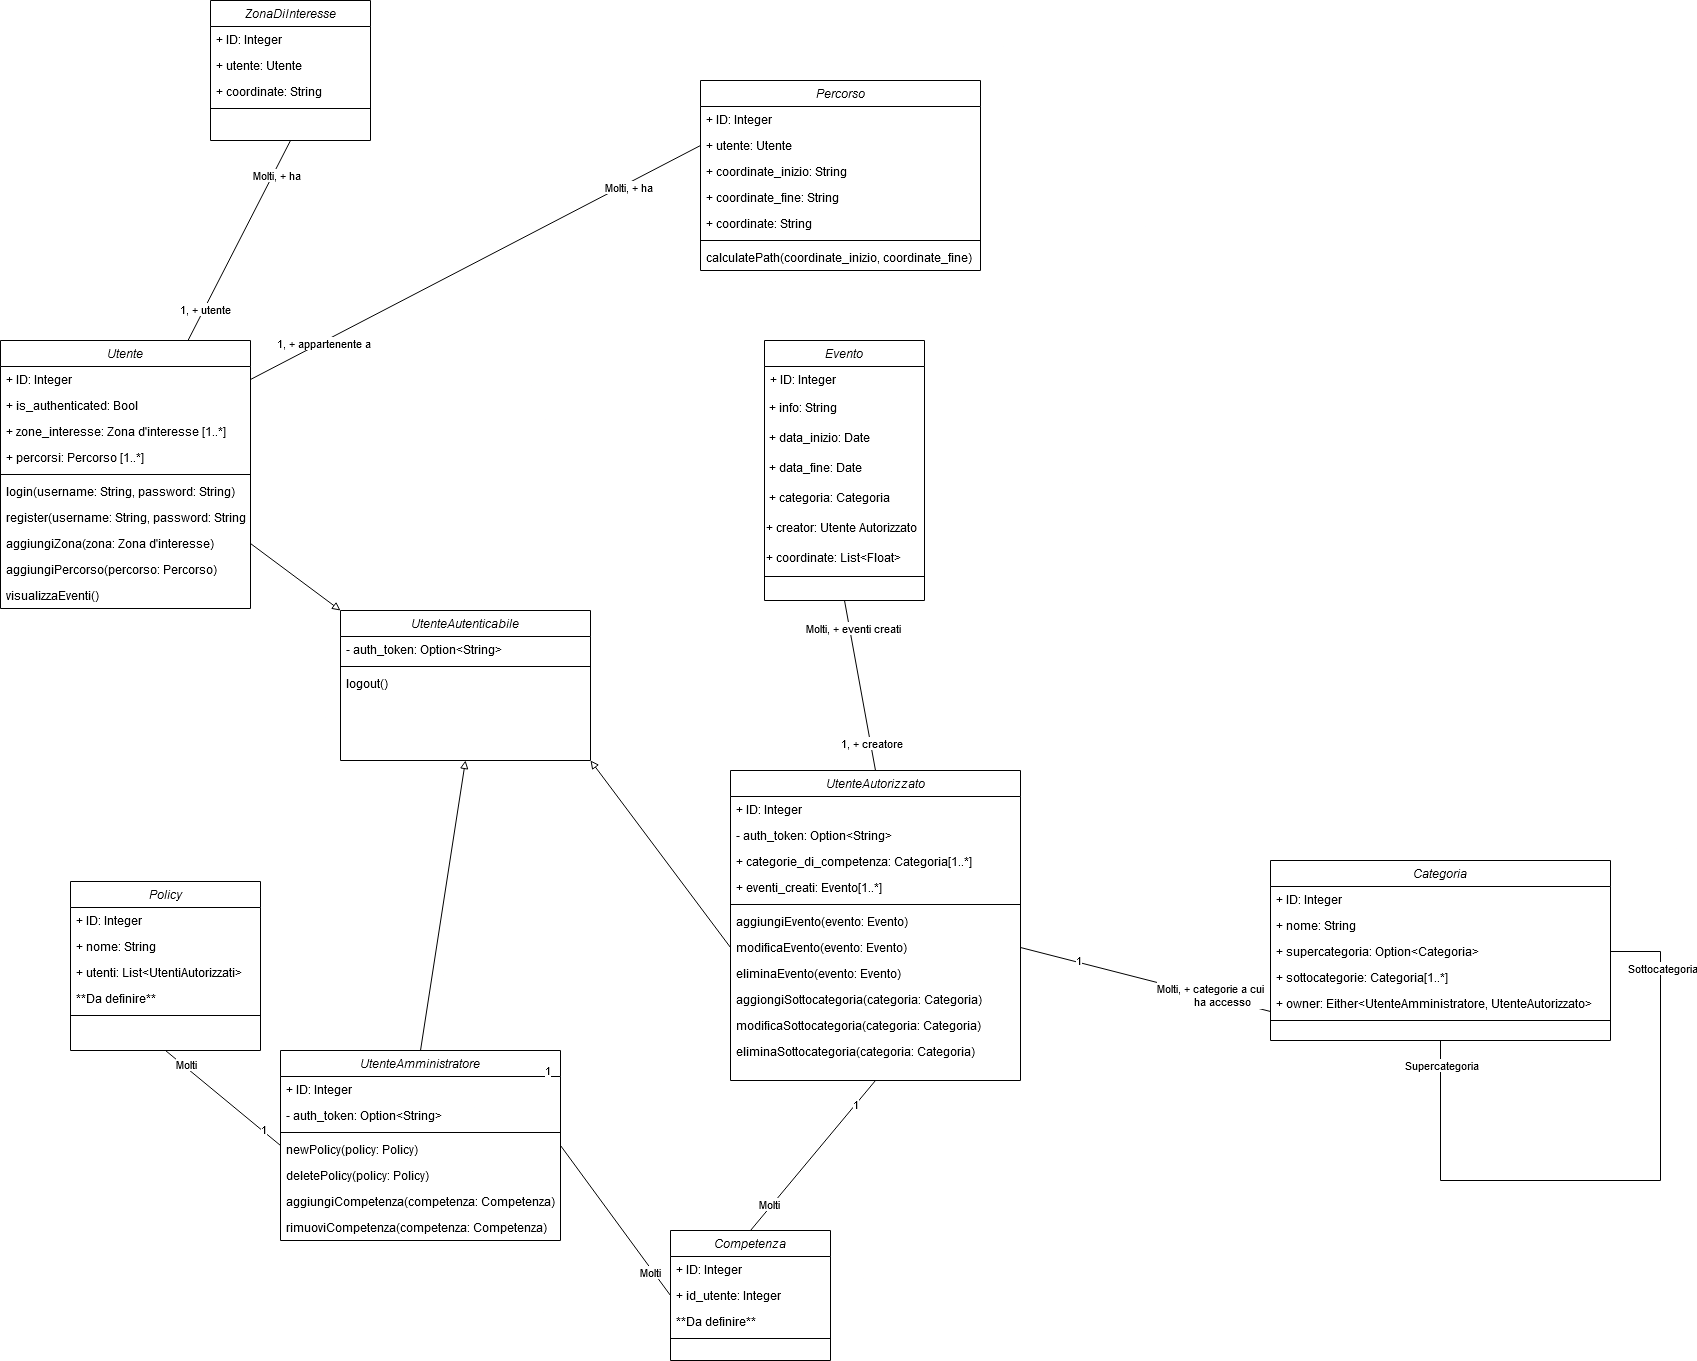
\includegraphics[width=1\textwidth]{Images/class_diagram.png}
    \caption{Diagramma delle classi}
    \label{fig:class-diagram}
\end{figure}

\clearpage

\section{Contstraints con OCL}
\index{Constraints con OCL}  

\subsection{Utente}
\index{Utente}

\begin{verbatim}
context Utente
    inv: self.zone_interesse -> forAll(z | z.utente == self)
    inv: self.percorsi -> forAll(p | p.utente == self)
    inv: self.auth_token.isEmpty() == self.is_authenticated
\end{verbatim}

\subsection{Utente autenticabile}
\index{Utente autenticabile}

\begin{verbatim}
context UtenteAutenticabile::login(_username, _password)
    pre: self.is_authenticated == false
    post: !self.auth_token.isEmpty()

context UtenteAutenticabile::deauthenticate()
    pre: self.is_authenticated == true
    post: self.auth_token.isEmpty()

context Utente::aggiungiZona(zona: ZonaDiInteresse)
    post: self.zone_interesse -> include(zona)

context Utente::aggiungiPercorso(percorso: Percorso)
    post: self.percorsi -> include(percorso)
\end{verbatim}

\subsection{Evento}
\index{Evento}

\begin{verbatim}
context Evento
    inv: self.creator.categorie_di_competenza -> includes(self.categoria)
    inv: self.creator.eventi_creati -> includes(self)
    inv: self.data_inizio <= self.data_fine
    inv: !self.info.isEmpty()
\end{verbatim}

\subsection{Categoria}
\index{Categoria}

\begin{verbatim}
# l'Admin può creare solo categorie "root" con profondità massima di 1
    inv: if instanceof(self.owner) == UtenteAmministratore:
        self.supercategoria == None || self.supecategoria->forAll(s | s.supercategoria == None)

# ogni sottoalbero di categorie deve avere una radice in un nodo "Root"
\end{verbatim}

\clearpage

\subsection{Utente Autorizzato}
\index{Utente Autorizzato}

\begin{verbatim}
context UtenteAutorizzato
    inv: self.eventi_creati -> forAll(e | e.creator == self)
    inv: self.categorie_di_competenza -> forAll()

context UtenteAutorizzato::aggiungiEvento(evento: Evento)
    post: self.eventi_creati -> include(evento)

context UtenteAutorizzato::aggiungiSottocategoria(categoria: Categoria)
    pre: !categoria.supercategoria.isEmpty()
    pre: self.categorie_di_competenza -> includes(categoria.supercategoria)
    post: self.categorie_di_competenza -> includes(categoria)
    post: categoria.owner == self

context UtenteAutorizzato::eliminaSottocategoria(categoria: Categoria)
    pre: self.categorie_di_competenza -> includes(categoria)
    pre: instanceof(categoria.owner) != UtenteAutorizzato
    post: self.categorie_di_competenza -> !includes(categoria)

context UtenteAutorizzato::modificaSottocategoria(categoria: Categoria)
    pre: self.categorie_di_competenza -> includes(categoria)
    pre: instanceof(categoria.owner) != UtenteAmministratore
    post: self.categorie_di_competenza -> includes(categoria.supercategoria)
    post: categoria.owner == categoria@pre.owner

context UtenteAutorizzato::aggiungiEvento(evento: Evento)
    post: self.categorie_di_competenza -> includes(evento.categoria)
    post: self.eventi_creati -> includes(evento)
    post: evento.creator == self

context UtenteAutorizzato::modificaEvento(evento: Evento)
    pre: evento.creator == self
    post: evento.creator == self

context UtenteAutorizzato::eliminaEvento(evento: Evento)
    pre: evento.creator == self
    post: self.eventi_creati -> !includes(evento)
\end{verbatim}


\end{document}